% Content for Chapter 5, Section 5.6 — pulled in by chapters/05-system-design.tex
\subsection{مكوّنات الخدمة}

تضمّ طبقة التطبيق في هذه الخدمة خدمة واحدة، ويقع معظم التعقيد في طبقة البنية التحتية، لأن التسجيل عملية يقودها نظام خارجي يُجيب لاحقاً بإشعار غير مضمون الوصول. ويعرض الشكل~\ref{fig:comp-03} مكوّنات الخدمة وروابطها الخارجية.

\begin{figure}[htbp]
  \centering
  % 2.20:1 — full width is ~30% of the text block, so it places inline.
  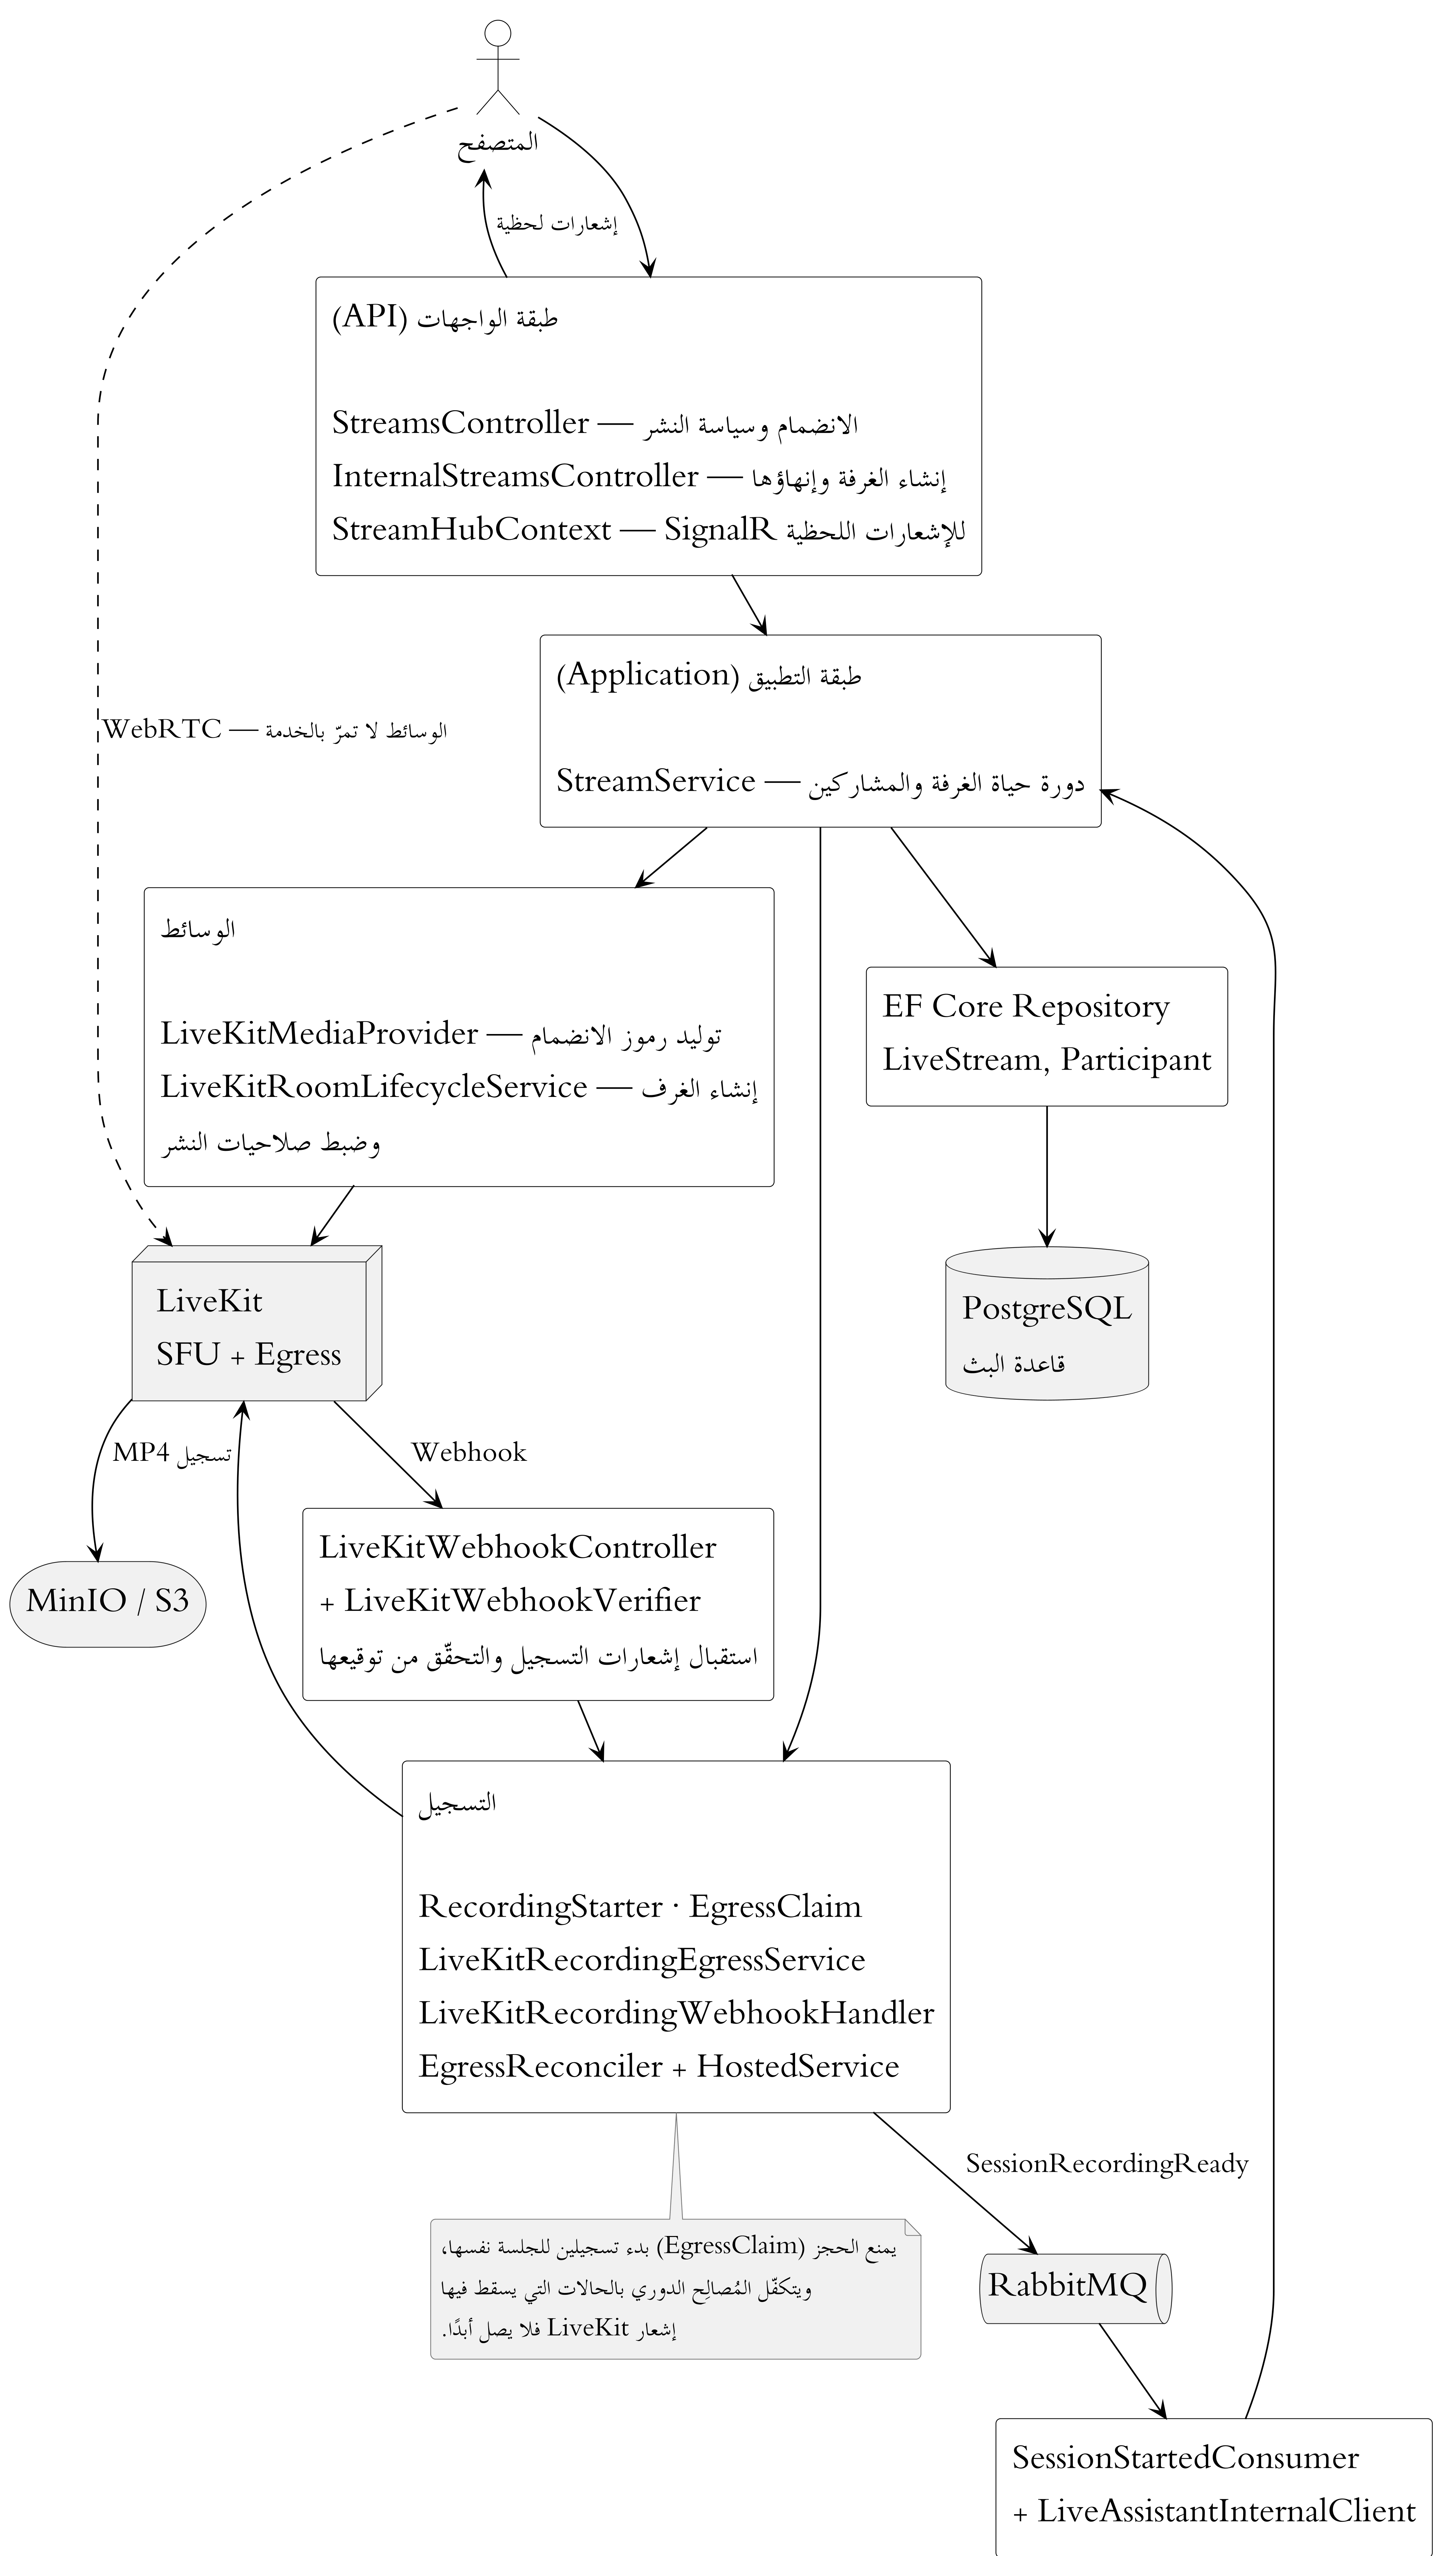
\includegraphics[width=\textwidth,height=0.8\textheight,keepaspectratio]{figures/comp-03-streaming.png}
  \caption{مخطط مكوّنات خدمة البث.}
  \label{fig:comp-03}
\end{figure}

ولا تمرّ الوسائط بالخدمة؛ إذ يتّصل المتصفّح بخادم \en{LiveKit} مباشرة عبر \en{WebRTC}، وتقتصر مهمّة الخدمة على إصدار رمز انضمام محدود الصلاحيات يحدّد ما يُسمح لصاحبه بنشره من صوت وصورة. ويمنع هذا الفصل تحوّل الخدمة إلى عنق زجاجة عند ارتفاع عدد المشاركين.

\subsection{نموذج البيانات}

يضمّ نموذج البيانات خمسة كيانات يعرضها الشكل~\ref{fig:erd-03}: البثّ الحيّ ومشاركوه، ورسائل المحادثة والأسئلة والتفاعلات المرافقة للجلسة.

% [H]: pinned under the paragraph that introduces it. Portrait at 0.90:1, so
% full width would be ~79% of the text block and could not share the page.
\begin{figure}[H]
  \centering
  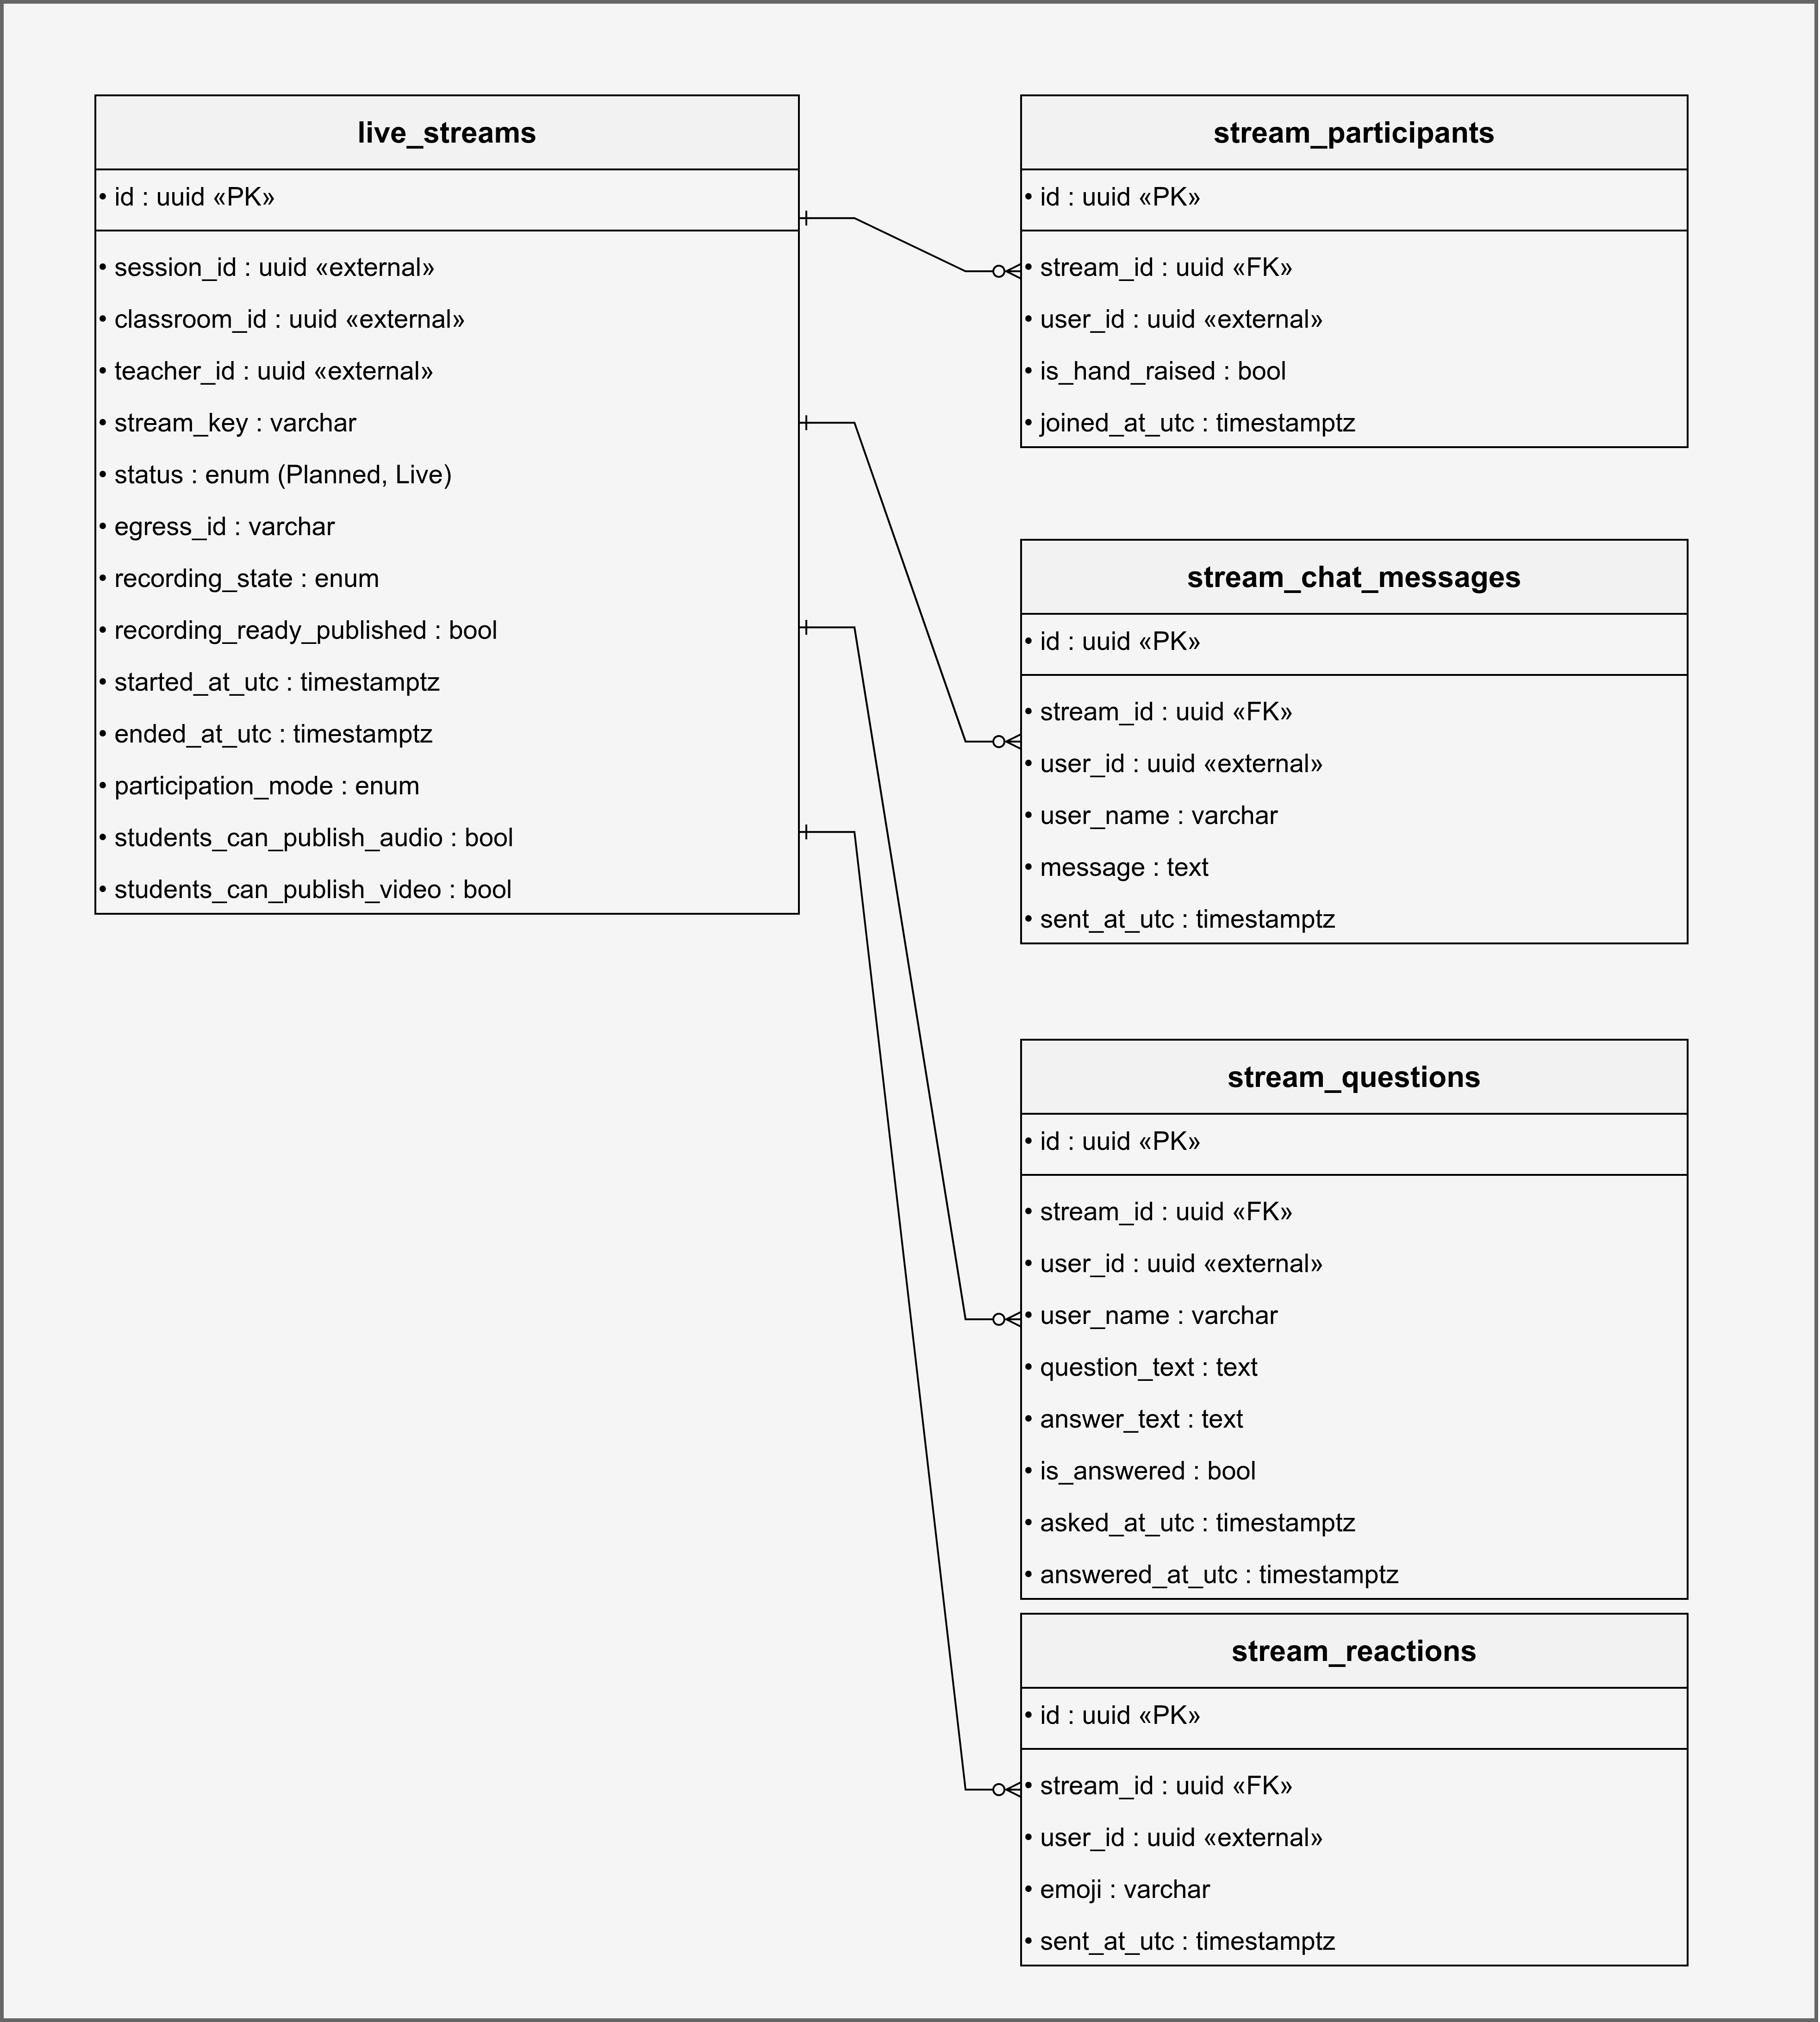
\includegraphics[width=0.55\textwidth,height=0.8\textheight,keepaspectratio]{figures/erd-03-streaming.png}
  \caption{مخطط الكيانات والعلاقات لخدمة البث.}
  \label{fig:erd-03}
\end{figure}
